\documentclass[aps,pra,reprint,groupedaddress]{revtex4-1}
%\documentclass[aps,prl,preprint,superscriptaddress]{revtex4-1}
%\documentclass[aps,prl,reprint,groupedaddress]{revtex4-1}

\usepackage{graphicx}
\usepackage{amsmath}

% You should use BibTeX and apsrev.bst for references
% Choosing a journal automatically selects the correct APS
% BibTeX style file (bst file), so only uncomment the line
% below if necessary.
%\bibliographystyle{apsrev4-1}

\begin{document}

\title{Phase dependent ionization of Rydberg atoms in static fields}
\author{Eric Magnuson}
\email[]{edm5gb@virginia.edu}
\author{T. F. Gallagher}
\email[]{tfg@virginia.edu}
\affiliation{University of Virginia, Department of Physics}
\date{\today}

\begin{abstract}
Using a laser intensity modulated synchronously with a 15.9 GHz microwave field we have examined laser excitation of Li atoms to the vicinity of the ionization limit in the presence of the microwave field and a parallel static field. The static field breaks the symmetry of ionization in the two microwave half cycles, and as the intensity modulated laser beam is delayed relative to the microwave field, maxima in the ionization are observed every microwave field cycle, not every half cycle, as in the absence of the static field. When the laser is tuned below the ionization limit there is an unexpected phase reversal of the modulation in the ionization, the origin of which is clarified by a classical model.
\end{abstract}

\pacs{}

\maketitle

\section{\label{sec:intro}Introduction}

Exposing atoms and molecules to the combination of a near infrared (NIR) laser pulse and the extreme ultraviolet (XUV) attosecond pulse train (APT) generated from it has proven to be a fruitful probe of ultrafast dynamics in atoms and molecules \cite{Krausz}. Ionization of He by the combination of a strong NIR field and a synchronized XUV APT provides an excellent example \cite{Johnsson, Ranitovic, Tong}.  In these experiments the XUV photons are not energetic enough to ionize the He, but in combination with the correct phase of the NIR field their absorption leads to ionization. While this process can be described in quantum-mechanical terms \cite{Johnsson, Ranitovic, Tong, Zhong}, a simple classical picture of the process is as follows. A photon in the XUV pulse creates a photoelectron moving away from the He$^+$ ion, and as the photoelectron leaves the ion it receives a momentum kick from the NIR field. The momentum transfer from the NIR field is greatest just after the photoelectron is created, when it is near the He$^+$ and has a high velocity. Thus the phase of the NIR field at which the XUV excitation occurs is important. If the phase of the NIR field is such that enough energy is added to the photoelectron, ionization occurs, otherwise not. In a typical experiment ionization of an atom or molecule is monitored as the APT is delayed relative to the NIR pulse so that the attosecond pulses coincide with different phases of the NIR field. Since an attosecond  pulse is generated on each half cycle of the NIR field, and each attosecond pulse generates photoelectrons moving parallel and antiparallel to the NIR field, ionization by the combined NIR and attosecond pulses is equally likely on both half cycles of the NIR field. The result is a delay dependent ionization signal with a period half the NIR period.

If the process being probed is different for the positive and negative half cycles of the NIR pulse, such as ejection of electrons in a specific direction, and the angular distribution of a bound electron distribution, the asymmetry cannot be detected by the usual APT, which has an XUV pulse every NIR half cycle. In quantum mechanical terms the usual APT contains only odd harmonics of the NIR field, precluding the observation of such angular effects \cite{Zhong}. Such an asymmetry can be detected by a single attosecond pulse (SAP) which samples only one half cycle of the NIR field or by an APT with one pulse per NIR field cycle. Such an APT contains both even and odd harmonics of the NIR field, leading to observable angular effects \cite{Zhong}. An APT with one pulse per NIR field cycle can be generated using the fundamental and second harmonic of the NIR field \cite{Mauritsson}. This approach has recently been used to observe the directional dissociation of D$_2^+$ \cite{Singh}.

The experiments described above are examples of probing dynamics using the combination of a strong low frequency field and a synchronously modulated high frequency field. A different example is exploring the photoionization of atoms in the presence of a strong microwave field by using a visible laser intensity modulated at twice the microwave frequency \cite{Carrat}. As in the NIR-APT experiments, depending upon the phase of the microwave field at which laser excitation occurs, the microwave field adds energy to or subtracts it from the photoelectron, resulting in a phase dependent ionization probability, even if the laser is tuned above the ionization limit \cite{Shuman}. Since the laser pulse generates photoelectrons moving both with and against the microwave field, neither half cycle of the microwave field is favored as the modulated laser pulse is delayed relative to the microwave field, and the ionization signal varies sinusoidally, with half the microwave period, as in the laser experiments described above.

Here we describe our experiment in which we break the symmetry of the two microwave half cycles by the addition of a static field polarized in the same direction. The potential of an atom in a static electric field is shown schematically in Fig.~\ref{fig:CoulMW}. A laser pulse produces an equal number of photoelectrons leaving the ion core in the uphill and downhill directions, as shown by the double headed arrow in Fig.~\ref{fig:CoulMW}. At one phase of the microwave field all the electrons receive an upfield momentum kick and at the opposite phase they all receive a downhill kick. To probe this process, which is asymmetric in the two microwave half cycles, we use a visible laser intensity modulated at (not twice) the microwave frequency. We observe the expected modulation in the ionization signal as the modulated laser pulse is delayed relative to the microwave field. As expected, the modulation in the ionization signal changes sign when the static field is reversed. Unexpectedly, when the laser is tuned slightly below the limit we observe an unexpected additional reversal of the modulation as the static field is varied.

\begin{figure}
	\includegraphics[width=3.3in]{CoulMW}
	\caption{Photoelectrons produced by the 819-nm laser in the combined Coulomb and static fields. Both the laser and the static field are polarized along the z-axis. Photoelectrons leave the ion core moving both to the left and to the right, which we refer to as ``uphill'' or ``downhill'' electrons, respectively. The inset shows the z-polarized microwave field experienced by the electrons and the direction of the static field, also oriented along the z-axis.}
	\label{fig:CoulMW}
\end{figure}
In the sections which follow we describe the experimental approach, present our observations and a classical model of the process.

\section{\label{sec:exp} Experimental approach}

Li atoms in a collimated thermal beam pass through a microwave cavity, where they are excited to a high lying Rydberg state or the continuum by three laser pulses, via the route $2s \xrightarrow{\text{670 nm}} 2p \xrightarrow{\text{610 nm}} 3d \xrightarrow{\text{819 nm}} nf, \epsilon f$, as shown by Fig.~\ref{fig:ELev}. The 610-nm beam is counterpropagating to the Li beam, and the 670-nm and intensity modulated 819-nm beams cross it at a right angle, forming a 1 mm$^3$ excitation region. This region is at an anti-node of the microwave electric field of the 15.9 GHz Fabry-Perot cavity. The laser excitation occurs in the presence of the vertically linearly polarized microwave field and a parallel static field. The interaction region is enclosed on top, bottom and two sides by aluminum plates. Combined with the two Fabry-Perot mirrors, this forms a 10-cm cubic enclosure. Bias voltages can be applied independently to each plate and mirror to control static fields in the interaction region.

\begin{figure}
	\includegraphics[width=3.3in]{ELevel}
	\caption{Energy level diagram for exciting a thermal beam of Li atoms from their ground state to high lying Rydberg states or the continuum via the route $2s \xrightarrow{\text{671 nm}} 2p \xrightarrow{\text{610 nm}} 3d \xrightarrow{\text{819 nm}} nf, \epsilon f$. The $2s \rightarrow 2p \rightarrow 3d$ excitation is driven by two simultaneous 20 ns dye laser pulses with 10 GHz linewidths. The final $3d \rightarrow nf, \epsilon f$ excitation occurs after the dye laser pulses, and is driven by a 20 ns pulse from an amplified, intensity modulated 819-nm laser. The 819-nm and 670-nm beams intersect the Li beam perpendicular to it, while the 610-nm beam propagates counter to the Li beam, creating a 1 mm$^3$ interaction region.}
	\label{fig:ELev}
\end{figure}

The 300 ns long microwave pulse into cavity begins 240 ns before the first laser pulse and ends 20 ns after the last laser pulse. Synchronous with the microwave pulse, balanced positive and negative voltage pulses are applied to plates above and below the interaction region to produce a vertical static field in the interaction region. We term this field the static field to distinguish it from the field pulse used for field ionization. The 20 ns long 610-nm and 670-nm laser pulses are simultaneous and are immediately followed by an 819-nm pulse of 20 ns duration.

One microsecond after the microwave and static fields are turned off we field ionize surviving atoms in Rydberg states within 100 GHz of the ionization limit by applying a negative voltage pulse to the plate below the interaction region. If the static and microwave fields are left on, there are no bound atoms after 1 $\mu$s, and it is for this reason that these fields are turned off. The time delay before the field ionization pulse allows any free electrons produced to disperse. Electrons resulting from field ionization are driven to a microchannel plate (MCP) assembly above the interaction region, and the resulting MCP signal, $S_{Ryd}$, is captured with a gated integrator and recorded in a computer.

The signal of interest is the number of atoms surviving the combined static and microwave fields, in particular its dependence on the phase of the microwave field at which the atoms are excited by the 819-nm laser.
To characterize this phase, or the time delay, we define the microwave field in the cavity as
\begin{equation}
E(t) =E_{mw}\sin{\omega t},
\end{equation}
where $E_{mw}$ is the amplitude of the microwave field, and $\omega$ is the microwave angular frequency; $\omega/2\pi=$15.9 GHz. The 819-nm laser intensity $I(t$) is given by
\begin{equation} \label{eq:AMLaser}
I(t) =\frac{I_0}{2}(1+\cos{(\omega (t-t_0)}).
\end{equation}
where $I_0$ is the peak optical intensity, and $t_0$ is the time delay introduced by the delay line in the 819-nm beam. With these definitions $t_0=0$ corresponds to the peak laser intensity's occurring at a zero crossing of the microwave field.

To make the measurement we delay the modulated 819-nm beam relative to the microwave field in the cavity, as shown in Fig.~\ref{fig:AMLaser}. For each delay $t_0$ we record the signal $S_{Ryd}$ for 1000 laser shots and then record a total excitation signal $S_{total}$ for 1000 laser shots. The $S_{total}$ signal is obtained by applying the field ionization pulse synchronously with the 819-nm laser pulse so as to collect electrons from both bound states and the continuum. Dividing $S_{Ryd}$ by $S_{total}$ yields the normalized signal
\begin{equation} \label{eq:norm}
S=\frac{S_{Ryd}}{S_{total}},
\end{equation}
which is the fraction of laser excited atoms left in bound states, and $1-S$ is the fraction ionized. All signals reported in this paper are normalized according to Eq.~\ref{eq:norm}.

\begin{figure}
	\includegraphics[width=3.3in]{AMTiming}
	\caption{Temporal view of the microwave field (top) phase-locked with the amplitude modulated laser intensity (bottom). Inside the interaction region, the peak laser intensity occurs at the phase $\omega t_0$ of the microwave field and can be adjusted by an optical delay line.}
	\label{fig:AMLaser}
\end{figure}

\subsection{\label{sec:dye} 670 and 610-nm Dye Lasers}

We use two dye lasers at 670-nm and 610-nm to drive the $2s \rightarrow 2p$ and $2p \rightarrow 3d$ transitions, respectively. These dye lasers are pumped by a Quantronix Darwin Nd:YLF laser, which produces 30 mJ, 100-ns (FWHM) pulses at a 1-kHz repetition rate. Using a Pockels cell (PC) and polarizing beam splitter (PBS), the first 20 ns segment of the pulse is picked off and split equally to pump the 670-nm and 610-nm lasers. A second PC and PBS directs the next 20-ns slice, from the peak of the pump pulse, to pump a dye amplifier for the 819-nm laser. The long trailing edge of the pump pulse is dumped.

The 670-nm dye laser has a Littman-style cavity and LDS-698 laser dye dissolved in ethanol as a lasing medium \cite{Littman}. The 610-nm laser has a H{\"a}nsch style cavity with Rhodamine-610 laser dye dissolved in ethanol \cite{Hansch}. Both lasers have linewidths (FWHM) of 10-GHz. To minimize unintended ionization from the $3d$ state, both lasers are attenuated to 2 $\mu J$ pulse energies before being directed to the vacuum chamber.

\subsection{\label{sec:ampmod} Intensity Modulated 819-nm Laser}

The production of the amplitude-modulated beam is shown in Fig.~\ref{fig:pll}. Labels in parentheses in the following paragraphs refer to labels in the figure. The 819-nm beam is produced using two external-cavity diode lasers, a Toptica DL-100 (DL-100) and a DL-Pro (DL-Pro). The lasers are tuned such that their frequencies are separated by the 15.9 GHz microwave frequency, and the two beams are overlapped on a 50:50 beamsplitter (BS) to produce the intensity modulated beam. One output from the BS is directed to a high speed photodetector (PD) to detect the microwave frequency beat note and deliver the signal to a phase-locked-loop. The second output of the BS provides 30 mW of intensity modulated light, which is passed through a tapered amplifier (TA) and a dye amplifier (DA). The Toptica TA increases the power to 800 mW. The DA is pumped by the 20-ns square pulse picked from the peak of the Nd:YLF laser pulse. We use LDS-819 dissolved in ethanol as the amplification medium. The final result is a 20 ns long, 6 $\mu$J pulse of sinusoidally intensity-modulated 819-nm light, which is sent to the interaction region. Although the 819-nm beam is produced by two diode lasers, we shall refer to this arrangement as the 819-nm laser. Its center frequency is the average of the two diode laser frequencies.

\begin{figure}
	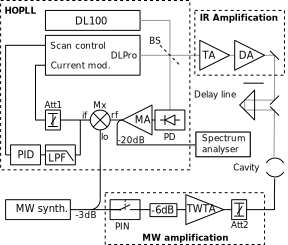
\includegraphics[]{beatexp}
	\caption{Schematic showing how the intensity modulated 819-nm laser is produced and locked to the microwave frequency, as well as how both the laser and microwave fields are delivered to the interaction region. The intensity modulated IR laser is generated by overlapping the DL-Pro and DL-100 laser beams on a beamsplitter (BS). One output is amplified through a tapered amplifier (TA) and dye amplifier (DA) and sent to the interaction region. The second is mixed with half the output of the microwave synthesizer to lock the intensity modulation to the microwaves using the Heterodyne Optical Phase Locked Loop (HOPPL). The other half of the synthesizer's output is formed into pulses by the PIN switch and amplified by the traveling wave tube amplifier (TWTA) before injection into the microwave cavity.}
	\label{fig:pll}
\end{figure}

The intensity modulation of the laser is locked to the microwave frequency with a heterodyne optical phase-locked-loop (HOPLL). The locking is driven by a ``fast'' feedback to the current input of the DL-Pro, and a ``slow'' feedback to its scan input. To produce an error signal, the beat note from the PD is amplified (MA) and mixed (Mx) with the output of the microwave source (MW synth.). The error signal is passed through a variable attenuator (Att1) and then connected to the Current input of the Toptica DL-Pro, providing a lock between the laser intensity modulation and the microwave field that lasts for several minutes.

To achieve longer lock times, on the order of hours, we use a Toptica PID-110 (PID) servo unit to drive the scan input of the DL-Pro. The ``fast'' current lock described above is primarily lost due to the lasers' drifting out of the range that the DL-Pro current input can correct. To circumvent this problem the error signal is sent through a low-pass filter (LPF), processed through the PID, and fed to the Scan input, which corrects long term drifts in the modulation frequency. This leaves only high-frequency errors for the ``fast'' loop to correct. The phase lock is robust, typically lasting more than three hours.

Once locked, the phase of the intensity modulation at the BS is constant relative to the microwave field, and its phase relative to the microwave field in the interaction region is controlled by the delay $t_0$ introduced by the optical delay line, which consists of a retro-reflector mounted on a translation stage, as shown in Fig~\ref{fig:pll}. Using it we are able to extend the path length of the modulated laser beam by several microwave wavelengths.

\subsection{\label{cavity} Microwave Apparatus}

A Hittite HMC T-2100 synthesizer (MW synth.) tuned to the 15.9-GHz resonance of the microwave cavity is our microwave source. It produces 9 dBm (8 mW) of power, and a splitter diverts half of the power to the microwave mixer (Mx) to generate the error signal for the HOPLL. The other half of the signal is formed into 300-ns pulses by a microwave switch (PIN), and then amplified by a Hughes 8020H04F traveling-wave-tube-amplifier (TWTA). Between the TWTA and the cavity, there is a 0 to 50 dB variable attenuator (Att2), allowing us to control the intensity of the pulse incident on the microwave cavity.

The microwave Fabry-Perot cavity is composed of two brass spherical mirrors. These mirrors have 10 cm radii of curvature, 10.2 cm diameters, and an on axis separation of 7.83 cm. The 15.9 GHz resonance is the TEM$_{008}$ mode of the cavity, with a quality factor $Q=3600$. We are able to determine the field inside the cavity with an uncertainty of 15\%. The 300 ns long microwave pulses are injected into the cavity 280 ns before the end of the last laser pulse and are turned off 20 ns after the end of the laser pulse. When the microwaves are turned off, the microwave field decays with a time constant of 72 ns.

\subsection{\label{fields} Static Fields}

This experiment depends on the detection of atoms in long lived Rydberg states close to the ionization limit. To prevent atoms in these states from ionizing before detection, we minimize the ambient static field in the interaction region. We accomplish this by surrounding the interaction region on two sides with the brass microwave cavity mirrors, and on the remaining two sides, top, and bottom with polished aluminum plates. A voltage can be applied independently to each plate or mirror, allowing us to compensate ambient static fields in every direction. We measure the depressed ionization limit (DIL) to minimize stray fields and estimate the residual static field. In this manner, we determine the remaining static field to have a magnitude of 1.5 mV/cm. This results in a DIL 7 GHz below the the zero field ionization limit. This value for the DIL remained constant for all the experiments discussed in this paper.

To apply a vertical static field to the interaction region during excitation of Rydberg states we use a two-channel arbitrary waveform generator (AWG) to apply 300-ns square pulses of the same magnitude and opposite polarity to the top and bottom bias plates. This square pulse is synchronous with the microwave pulse. One microsecond after the final laser pulse, the same AWG applies a -900 mV voltage step to the bottom plate to produce a -0.65 V/cm ionization field, ionizing high-lying states and driving the resulting electrons toward the MCP stack.

\section{\label{results} Results}

The delay scans of Fig.~\ref{fig:fph} show many of the important features of our observations. They are the result of detecting the Rydberg field ionization signal while scanning the time delay $t_0$ with the center frequency of the 819-nm laser tuned 2 GHz above the DIL (5 GHz below the zero-field ionization limit), in the presence of a microwave field of amplitude $E_{mw}=4$ V/cm and several values of the static field. All of the data reported in this paper were taken with this microwave field. Instead of plotting the signals vs the time delay $t_0$ we plot them vs the phase shift $\phi_0=\omega t_0$ of the 819-nm laser intensity envelope relative to the microwave field, as shown by Fig.~\ref{fig:AMLaser}. We do not know the absolute phase $\phi_0$, so we assign the phase $\phi_0=\pi/6$ to the phase at which the maximum number of Rydberg atoms is observed with the laser tuned 2 GHz above the DIL and static field $E_s = 14$ mV/cm. All delay scans follow this convention, and all signals are normalized according to Eq. (\ref{eq:norm}).

\begin{figure}
	\includegraphics[width=3.3in]{FieldPhase}
	\caption{Rydberg state signal as the phase delay is scanned for various values of $E_S$. The central laser frequency is tuned to 2 GHz above the DIL. The vertical scale is normalized such that 1 is the total number of electrons excited by the 819-nm laser. When no static field is applied, there is no observed phase modulation. As the static field in increased, the phase dependence in the signal grows and then lessens as the total mean signal decreases. The experimental data are shown in grey, while the solid sinusoidal curves trace the best fit to Eq. (\ref{eq:modfit}). The traces at $+7.2$ (solid) and $-7.2$ (dashed) mV/cm show reversing the static field inverts the amplitude of the phase modulation.}
	\label{fig:fph}
\end{figure}

In Fig.~\ref{fig:fph} we show the results obtained with $E_{s}=$ 0, 7.2, -7.2, 36.0 and 108.0 mV/cm, all in the vertical direction. The results are in accord with our expectations. First, with zero static field, there is no observed phase dependence, while at 7.2 mV/cm there is a 5\% peak to peak (PP) modulation. A modulation in the ionization can only be observed when a static field is applied in addition to the microwave field. Equally important, when the static field is reversed, to -7.2 mV/cm, the phase dependent modulation reverses sign, as shown by Fig.~\ref{fig:fph}. As $E_s$ is increased further, both the mean signal and the peak to peak modulation decrease, and the delay at which the detected signal is greatest shifts somewhat at higher static field,

While the addition of a static field in the vertical direction breaks the symmetry of the two microwave half cycles, a horizontal field should not, and in Fig.~\ref{fig:CircleDelay} we show delay scans taken in 14 mV/cm vertical and horizontal static fields. The laser is tuned 14 GHz below the DIL. As shown in Fig.~\ref{fig:CircleDelay}, no modulation is observed with a horizontal static field, and the observed modulation changes sign when the direction of the vertical static field is reversed.

\begin{figure}
	\includegraphics[width=3.3in]{CircleDelay}
	\caption{Rydberg signal obtained vs phase delay for laser tuning 14 GHz below the DIL in three different 14 mV/cm static fields ($E_s$) oriented parallel and perpendicular to the z polarized microwave field. (a) $E_s$ in the $+\hat{z}$ (vertical) direction, (b) $E_s$ in the $+\hat{x}$ (horizontal) direction, and (c) $E_s$ in the $-\hat{z}$ (vertical) direction. There is no dependence on the delay with the static field perpendicular to the microwave field, as expected from the symmetry of the problem.}
	\label{fig:CircleDelay}
\end{figure}

With the laser tuned 2 GHz above the DIL we have taken extensive data, of which those shown in Fig.~\ref{fig:fph} are representative. To present these data in a more compact way we fit the observed phase scans to the sinusoidal form:
\begin{equation} \label{eq:modfit}
S = S_m \cos{[\phi_0 - \phi_S]} + S_0
\end{equation}
where $S_0$ is the phase average signal, and $S_m$ and $\phi_S$ are the amplitude and phase offset of the modulation. We constrain $\phi_S$ to lie in the range $0\leq \phi_S \leq \pi$, which results in the plots shown in Fig.~\ref{fig:DILP2}. As expected, $S_0$ decreases from $S_0=0.3$  as the magnitude of the static field is increased. the amplitude of the modulation $S_m$ is an odd function of the static field, reaching its maximal positive and negative values at $E_s=\pm 14$ mV/cm. Finally, the phase $\phi_S$ is approximately constant.

\begin{figure}
	\includegraphics[width=3.3in]{DILP2}
	\caption{(a) Peak to peak modulation $2 \cdot S_m$, (b) mean signal $S_0$, and (c) phase $\phi_S$ vs static field $E_s$ observed with the laser tuned 2 GHz above the DIL. These parameters are extracted by fitting delay scans such as those of Fig.~\ref{fig:fph} to Eq. (\ref{eq:modfit}) with the constraint $0 \leq \phi_S \leq \pi$. At zero static field, $E_s = 0$, the mean signal is at a maximum, and there is no modulation. We observe that modulation emerges as the magnitude of $E_S$ is increased from zero, reaching a peak at $E_S = \pm 14$ mV/cm. For $|E_s| > 14$ mV/cm the mean signal and modulation both decay toward zero. The phase is roughly identical for data collected at equal and opposite $E_S$, and there is a positive phase shift as the magnitude of $E_S$ is increased.}
	\label{fig:DILP2}
\end{figure}

As shown by Fig.~\ref{fig:DILM14}, when the 819-nm laser is tuned 14 GHz below the DIL, the average number of surviving atoms increases, as might be expected. Unexpectedly, with this laser tuning a small static field results in a modulation of opposite polarity to that seen in Fig.~\ref{fig:DILP2}. As the amplitude of the static field is raised, the modulation changes sign, and at static fields larger than $\pm 27$ mV/cm it has the same sign as seen in Fig.~\ref{fig:DILP2}. While the sign reversal relative to Fig.~\ref{fig:DILP2} at small static fields is surprising, the similarity at higher static fields is not.

\begin{figure}
	\includegraphics[width=3.3in]{DILM14}
	\caption{(a) Peak to peak modulation $2 \cdot S_m$, (b) mean signal $S_0$, and (c) phase $\phi_S$ vs static field $E_s$ observed with the laser tuned 14 GHz below the DIL. These parameters are extracted by fitting delay scans such as those of Fig.~\ref{fig:fph} to Eq. (\ref{eq:modfit}) with the constraint \textbf{[phi 0]} $0 \leq \phi_S \leq \pi$. At zero static field, we again observe the maximum mean signal, and there is no modulation. For small static fields, $|E_s|<27$ mV/cm, the modulation has the opposite sign to that shown in Fig.~\ref{fig:DILP2} and reaches its first peak at $E_S = \pm 14$ mV/cm. As the magnitude of the static field is increased modulation decreases and crosses zero at $E_S = \pm 27$ mV/cm. For $|E_s|> 27$mV/cm the modulation has the same sign as in Fig.~\ref{fig:DILP2}, reaching its maximum at $E_s= \pm 60$ mV/cm, and decreasing for higher magnitudes of the static field. A slight positive shift of the phase is observed as $|E_s|$ is increased.}
	\label{fig:DILM14}
\end{figure}

Finally, Fig.~\ref{fig:DILM30} shows the results for the laser tuned to DIL - 30 GHz. They resemble the DIL - 14 GHz case of Fig.~\ref{fig:DILM14}, except that there is no modulation for a finite field range, -20 mV/cm $<E_s<$ 20 mV/cm, around zero static field. The appearance of this new feature is due to the fact that the presence of a small static field plays a diminishing role as the laser is tuned progressively further below the limit. As a result, for small static fields we obtain the zero field result.

\begin{figure}
	\includegraphics[width=3.3in]{DILM30}
	\caption{(a) Peak to peak modulation $2 \cdot S_m$, (b) mean signal $S_0$, and (c) phase $\phi_S$ vs static field $E_s$ observed with the laser tuned 30 GHz below the DIL. These parameters are extracted by fitting delay scans such as those of Fig.~\ref{fig:fph} to Eq. (\ref{eq:modfit}) with the constraint $0 \leq \phi_S \leq \pi$. As in Figs.~\ref{fig:DILP2} and \ref{fig:DILM14}, there is a maximum in the mean signal at $E_s=0$. Unlike Figs.~\ref{fig:DILP2} and \ref{fig:DILM14}, modulation is not immediately observed for $E_s\neq 0$. Modulation is not observed until $E_s=\pm 30$ mV/cm, at which point it has the same sign as in Fig.~\ref{fig:DILM14}. It reaches its first maximum at $E_s = 50$ mV/cm, crosses zero at $E_s=\pm 65$ mV/cm, reaches its second maximum at $E_s = \pm 144$ mV/cm, and decays to zero as $|E_s|$ is further increased. The phase appears to be constant.}
	\label{fig:DILM30}
\end{figure}

\section{\label{sec:disc} Two Dimensional Classical Model}

To provide insight into the observed phase dependence in the number of detected atoms as well as the phase reversal observed when the laser is tuned below the DIL we have constructed a two-dimensional model of a classical Rydberg electron moving in the combined Coulomb (coul), static (s), and microwave (mw) fields. Expressed in atomic units, the equation of motion is:
\begin{equation}
\begin{aligned}
\ddot{\vec{r}} & = -\vec{E}_{coul}(\vec{r}) - \vec{E}_{s}(t) - \vec{E}_{mw}(t) \\
 & = -\frac{1}{r^2} \cdot \hat{r} - \Theta_s(t) \cdot E_{s} \cdot \hat{z} \\
 & \quad \quad - \Theta_{mw}(t) \cdot E_{mw} \sin{(\omega t + \phi_0)} \cdot \hat{z}.
\end{aligned}
\end{equation}
Here $\Theta_s$ and $\Theta_{mw}$ are envelopes describing the square wave turning off the static field and the exponential ring-down of the microwave field. Assuming the photoelectron is produced at time $t=0$ the field envelopes are given by
\begin{equation}
\begin{aligned}
\Theta_s(t \leq t_{off}) & = 0 & \Theta_s(t > t_{off}) & = 0 \\
\Theta_{mw}(t \leq t_{off}) & = 1 & \Theta_{mw}(t > t_{off}) & = e^{-(t-t_{off})/\tau_{mw}}. \\
\end{aligned}
\end{equation}

In laboratory units the microwave field amplitude is 4 V/cm, the frequency is 15.9 GHz, the microwave and static fields are turned off at $t_{off} = 20$ ns, and $\tau_{mw} = 80$ ns. The electron is launched at time $t=0$ starting from the periapsis of the highly elliptical Rydberg orbit with an initial energy $W_0$ and initial angular momentum $l_0 = \sqrt{3 \cdot (3+1)}$, corresponding to an $f$ state. The electron's orbit lies in the x-z plane, and initially it is in an elliptical orbit with its semi-major axis along the the +z or -z axis. In Fig.~\ref{fig:udo} we show the beginnings of two trajectories, A and B, which are initially on elliptical orbits. If the static field $E_s$ is in the +z direction, as shown, an electron launched on trajectory A is reflected back toward the ion by the static field, and we label it an ``uphill'' trajectory. An electron launched on trajectory B is a ``downhill'' trajectory. Both trajectories shown in Fig.~\ref{fig:udo} have angular momenta in the +y direction. As expected from the symmetry of the problem, the results we obtain are unchanged when the sign of the angular momentum is reversed.

\begin{figure}
	\includegraphics[width=3.3in]{UDO}
	\caption{Schematic showing the beginning of (A) ``uphill'' and (B) ``downhill'' electron orbits in the 2 dimensional simulation, with the ion core at $(x, z) = (0, 0)$. Given initial radius and velocity $r_0$ and $v_0$, downhill electrons are launched from $(0, -r_0)$, with velocity in the $-\hat{x}$ direction. Uphill electrons are launched from $(0, +r_0)$ with velocity along $+\hat{x}$. Both orbits shown have angular momentum aligned in the $+\hat{y}$ direction. In the absence of a static field, bound electrons make highly elliptical orbits with the semi-major axis along the z-axis. The field $E_S$ applies a force in the $+\hat{z}$ direction on electrons during their orbits.}
	\label{fig:udo}
\end{figure}

For computation, the vector equations are expressed in terms of Cartesian coordinates \{x,y,z\}. Including the initial conditions, the system of ordinary differential equations to integrate is:
\begin{equation}
\begin{aligned}
x(0) & = 0 \\
z(0) & = \pm r_0 \\
\dot{x}(0) & = \pm v_0 \\
\dot{z}(0) & = 0 \\
\ddot{x} & = -\frac{x}{(x^2 + z^2)^{3/2}} \\
\ddot{z} & = -\frac{z}{(x^2 + z^2)^{3/2}} - \Theta_s(t) \cdot E_s \\
 & \quad \quad \quad - \Theta_{mw}(t) \cdot E_{mw} \cdot \sin{(\omega t + \phi_0)} & & \\
\end{aligned}
\end{equation}

For each initial electron energy $W_0$ and static field $E_s$, electrons are launched at 200 microwave phases $\phi_0$ between 0 and $2\pi$, in the ``uphill'' and ``downhill'' directions. The equations of motion are integrated until the microwave field has decayed for 5 times the decay constant, that is until  $t=t_{off} + 5\tau_{mw}$. After this integration time, the final energy, $W_f = 1/2 v_f^2 - 1/r_f$, of the electron is recorded. Here $v_f$ and $r_f$ are the final speed and distance from the ion core of the electron.

An electron with a positive final energy escapes from the ion, while those with negative final energies remain bound and are detected. The detected signal as a function of phase is convolved with the intensity envelope of the laser to produce a simulated signal. The laser intensity profile is given by Eq. (\ref{eq:AMLaser}) with $\phi_0=\omega t_0$. The calculated signals are normalized in the same way as the experimental data. To provide the maximum insight into the origin of the observed signals we treat the uphill and downhill electrons separately, then add them to produce the calculated signal.
In Fig.~\ref{fig:2DW0} we show the results for $W_0 =$ 0, 36, and 100 mV/cm. These calculations should mimic the experimental results shown in Fig.~\ref{fig:DILP2}. We recall that the plots of Figs.~\ref{fig:DILP2}, \ref{fig:DILM14}, and \ref{fig:DILM30} were made by constraining $\phi_S$ to lie in the range $0 \leq \phi_S \leq \pi$, while in Fig.~\ref{fig:2DW0} $\phi_0$ covers a range of $2\pi$. As expected, with $E_s=0$ there are equal modulations in the electrons ejected uphill, the $+\hat{z}$ direction, and downhill, the $-\hat{z}$ direction. The maximum in the uphill (downhill) signal occurs at $\phi_0=\pi/6$ ($7\pi/6$), the phase at which the microwave field removes the most energy from an uphill (downhill) electron. Since the modulations are $\pi$ out of phase, they cancel in the detected signal. In a static field of 36 mV/cm most of the downhill electrons leave, with a few surviving at $\phi_0=7\pi/6$, the phase at which the microwave field removes the maximum amount of energy from a downhill electron. More uphill electrons survive as bound atoms at all phases, but they are much more likely to survive if $\phi_0=\pi/6$, the phase at which the microwave field extracts the most energy from an uphill electron. Adding the uphill and downhill signals yields a total signal with a peak at $\phi_0=\pi/6$. When the static field is increased to 100 mV/cm no electrons ejected downhill result in bound atoms; the entire detected signal is due to electrons launched uphill. Irrespective of the static field the maximum number of bound atoms from uphill electrons occurs at $\phi_0=\pi/6$. These calculations, which are in agreement with the model of Shuman et al. \cite{Shuman}, are why we fixed the phase of the maximum experimental signals at $\phi_0=\pi/6$.

\begin{figure}
	\includegraphics[width=3.3in]{Sim0}
	\caption{Calculated observed signal from our 2 dimensional model, with initial energy $W_0 = 0$ GHz, and $E_s =$ (a) 0, (b) 36, and (c) 100 mV/cm. The contributions from downhill and uphill electrons are in orange (dotted) and blue (dashed), respectively, with the total expected signal in green (solid). In (a) with $E_s = 0$ mV/cm, uphill and downhill signals have opposite phase dependence, resulting in a flat total signal. As the static field $E_s$ increases in (b) and (c), ionization of downhill electrons depresses their mean signal and modulation, and the total signal becomes dominated by contributions from uphill electrons.}
	\label{fig:2DW0}
\end{figure}

The surprising aspect of our data is the sign reversal of the modulation with increasing static field when the laser is tuned below the DIL, as seen in Figs.~\ref{fig:DILM14} and \ref{fig:DILM30}. Fig.~\ref{fig:2DW20} shows the results for $W_0 = -20$ GHz and $E_s = 0, ~7.2, ~100$ mV/cm. As for $W_0=0$, when $E_s=0$ there is no modulation when the uphill and downhill signals are summed. When $E_s= 7.2$ mV/cm the maximum in the number of bound atoms detected occurs at $\phi_0 = 7\pi/6$, not $\pi/6$, as in Fig.~\ref{fig:2DW0}. The calculated signal exhibits the same phase reversal seen in the experimental data of Figs.~\ref{fig:DILM14} and \ref{fig:DILM30}. Examining the uphill and downhill electron contributions separately shows the origin of the reversal. At $E_s = 7.2$ mV/cm many of the uphill electrons are left as bound electrons for all phases, with only a slight dependence on $\phi_0$. While fewer of the downhill electrons are left bound, the dependence on $\phi_0$ is much more pronounced, with a peak at $\phi_0=7\pi/6$, the phase at which the most energy is removed from a downhill electron by the microwave field. Combining the uphill and downhill signals results in a peak in the total detected signal at $\phi_0=7\pi/6$. When the static field is raised to 100 mV/cm essentially all the downhill electrons leave the ion, and the uphill electrons, which are most likely to remain bound when $\phi_0=\pi/6$, constitute almost the entire signal. In the presence of the larger static field the tuning slightly below the limit becomes equivalent to tuning to the limit in any static field. In sum, the model shows both the origins of the phase dependence and the unexpected reversal observed when the laser is tuned below the DIL.

\begin{figure}
	\includegraphics[width=3.3in]{SimM20}
	\caption{Calculated observed signal from our 2 dimensional model, with initial energy $W_0 = -20$ GHz, and $E_s =$ (a) 0, (b) 7.2, and (c) 100 mV/cm.. Downhill and uphill signals are in orange (dotted) and blue (dashed), respectively, with total signal in green (solid). As in Fig.~\ref{fig:2DW0}, in (a) with $E_s = 0$ mV/cm, combining the equal and opposite uphill and downhill signals results in a flat total signal. In (b) with $E_s = 7.2$ mV/cm, the downhill signal is diminished, but its phase dependence increases. The total signal shows a phase dependence shifted by $\pi$ from the $E_s=36$ mV/cm signal for $W_0 = 0$ GHz in Fig.~\ref{fig:2DW0}. In (c) with $E_s = 100$ mV/cm, downhill electrons almost all ionize, and the uphill signal dominates the total signal.}
	\label{fig:2DW20}
\end{figure}

\section{\label{sec:conc} Conclusion}

Excitation of Li atoms by a linearly polarized, intensity modulated laser to the vicinity of the ionization limit in the presence of a similarly polarized microwave field results in a variation in the number of ions produced which depends on the phase of the microwave field at which the laser excitation occurs. Since the laser ejects photoelectrons moving parallel and antiparallel to the microwave field, as the intensity modulated laser beam is delayed a maximum in the ionization is observed in each microwave half cycle. The experiment reported here demonstrates that the addition of a static field parallel to the microwave field breaks the symmetry of the two half cycles of the microwave field, so that more ionization is observed in one half cycle than the other. In addition, when the laser is tuned below the ionization limit an unexpected phase reversal of the modulation of the ionization signal is observed in low static fields, but the phase reverts to that observed above the ionization limit in higher static fields. These observations are in agreement with a classical description of the process.

\section{\label{sec:ack} Acknowledgments}

We are grateful to Vincent Carrat, who participated in the initiation of this work. This work has been supported by the U. S. Department of Energy, Office of Science, Office of Basic Energy Sciences under Award Number DE-FG02-97ER14786.

%\bibliography{static_field_bib}

\begin{thebibliography}{11}%
\makeatletter
\providecommand \@ifxundefined [1]{%
 \@ifx{#1\undefined}
}%
\providecommand \@ifnum [1]{%
 \ifnum #1\expandafter \@firstoftwo
 \else \expandafter \@secondoftwo
 \fi
}%
\providecommand \@ifx [1]{%
 \ifx #1\expandafter \@firstoftwo
 \else \expandafter \@secondoftwo
 \fi
}%
\providecommand \natexlab [1]{#1}%
\providecommand \enquote  [1]{``#1''}%
\providecommand \bibnamefont  [1]{#1}%
\providecommand \bibfnamefont [1]{#1}%
\providecommand \citenamefont [1]{#1}%
\providecommand \href@noop [0]{\@secondoftwo}%
\providecommand \href [0]{\begingroup \@sanitize@url \@href}%
\providecommand \@href[1]{\@@startlink{#1}\@@href}%
\providecommand \@@href[1]{\endgroup#1\@@endlink}%
\providecommand \@sanitize@url [0]{\catcode `\\12\catcode `\$12\catcode
  `\&12\catcode `\#12\catcode `\^12\catcode `\_12\catcode `\%12\relax}%
\providecommand \@@startlink[1]{}%
\providecommand \@@endlink[0]{}%
\providecommand \url  [0]{\begingroup\@sanitize@url \@url }%
\providecommand \@url [1]{\endgroup\@href {#1}{\urlprefix }}%
\providecommand \urlprefix  [0]{URL }%
\providecommand \Eprint [0]{\href }%
\providecommand \doibase [0]{http://dx.doi.org/}%
\providecommand \selectlanguage [0]{\@gobble}%
\providecommand \bibinfo  [0]{\@secondoftwo}%
\providecommand \bibfield  [0]{\@secondoftwo}%
\providecommand \translation [1]{[#1]}%
\providecommand \BibitemOpen [0]{}%
\providecommand \bibitemStop [0]{}%
\providecommand \bibitemNoStop [0]{.\EOS\space}%
\providecommand \EOS [0]{\spacefactor3000\relax}%
\providecommand \BibitemShut  [1]{\csname bibitem#1\endcsname}%
\let\auto@bib@innerbib\@empty
%</preamble>
\bibitem [{\citenamefont {Krausz}\ and\ \citenamefont {Ivanov}(2009)}]{Krausz}%
  \BibitemOpen
  \bibfield  {author} {\bibinfo {author} {\bibfnamefont {F.}~\bibnamefont
  {Krausz}}\ and\ \bibinfo {author} {\bibfnamefont {M.}~\bibnamefont
  {Ivanov}},\ }\href {\doibase 10.1103/RevModPhys.81.163} {\bibfield  {journal}
  {\bibinfo  {journal} {Rev. Mod. Phys.}\ }\textbf {\bibinfo {volume} {81}},\
  \bibinfo {pages} {163} (\bibinfo {year} {2009})}\BibitemShut {NoStop}%
\bibitem [{\citenamefont {Johnsson}\ \emph {et~al.}(2007)\citenamefont
  {Johnsson}, \citenamefont {Mauritsson}, \citenamefont {Remetter},
  \citenamefont {L'Huillier},\ and\ \citenamefont {Schafer}}]{Johnsson}%
  \BibitemOpen
  \bibfield  {author} {\bibinfo {author} {\bibfnamefont {P.}~\bibnamefont
  {Johnsson}}, \bibinfo {author} {\bibfnamefont {J.}~\bibnamefont
  {Mauritsson}}, \bibinfo {author} {\bibfnamefont {T.}~\bibnamefont
  {Remetter}}, \bibinfo {author} {\bibfnamefont {A.}~\bibnamefont
  {L'Huillier}}, \ and\ \bibinfo {author} {\bibfnamefont {K.~J.}\ \bibnamefont
  {Schafer}},\ }\href {\doibase 10.1103/PhysRevLett.99.233001} {\bibfield
  {journal} {\bibinfo  {journal} {Phys. Rev. Lett.}\ }\textbf {\bibinfo
  {volume} {99}},\ \bibinfo {pages} {233001} (\bibinfo {year}
  {2007})}\BibitemShut {NoStop}%
\bibitem [{\citenamefont {Ranitovic}\ \emph {et~al.}(2010)\citenamefont
  {Ranitovic}, \citenamefont {Tong}, \citenamefont {Gramkow}, \citenamefont
  {De}, \citenamefont {DePaola}, \citenamefont {Singh}, \citenamefont {Cao},
  \citenamefont {Magrakvelidze}, \citenamefont {Ray}, \citenamefont
  {Bocharova}, \citenamefont {Mashiko}, \citenamefont {Sandhu}, \citenamefont
  {Gagnon}, \citenamefont {Murnane}, \citenamefont {Kapteyn}, \citenamefont
  {Litvinyuk},\ and\ \citenamefont {Cocke}}]{Ranitovic}%
  \BibitemOpen
  \bibfield  {author} {\bibinfo {author} {\bibfnamefont {P.}~\bibnamefont
  {Ranitovic}}, \bibinfo {author} {\bibfnamefont {X.~M.}\ \bibnamefont {Tong}},
  \bibinfo {author} {\bibfnamefont {B.}~\bibnamefont {Gramkow}}, \bibinfo
  {author} {\bibfnamefont {S.}~\bibnamefont {De}}, \bibinfo {author}
  {\bibfnamefont {B.}~\bibnamefont {DePaola}}, \bibinfo {author} {\bibfnamefont
  {K.~P.}\ \bibnamefont {Singh}}, \bibinfo {author} {\bibfnamefont
  {W.}~\bibnamefont {Cao}}, \bibinfo {author} {\bibfnamefont {M.}~\bibnamefont
  {Magrakvelidze}}, \bibinfo {author} {\bibfnamefont {D.}~\bibnamefont {Ray}},
  \bibinfo {author} {\bibfnamefont {I.}~\bibnamefont {Bocharova}}, \bibinfo
  {author} {\bibfnamefont {H.}~\bibnamefont {Mashiko}}, \bibinfo {author}
  {\bibfnamefont {A.}~\bibnamefont {Sandhu}}, \bibinfo {author} {\bibfnamefont
  {E.}~\bibnamefont {Gagnon}}, \bibinfo {author} {\bibfnamefont {M.~M.}\
  \bibnamefont {Murnane}}, \bibinfo {author} {\bibfnamefont {H.}~\bibnamefont
  {Kapteyn}}, \bibinfo {author} {\bibfnamefont {I.}~\bibnamefont {Litvinyuk}},
  \ and\ \bibinfo {author} {\bibfnamefont {C.~L.}\ \bibnamefont {Cocke}},\
  }\href {http://stacks.iop.org/1367-2630/12/i=1/a=013008} {\bibfield
  {journal} {\bibinfo  {journal} {New Journal of Physics}\ }\textbf {\bibinfo
  {volume} {12}},\ \bibinfo {pages} {013008} (\bibinfo {year}
  {2010})}\BibitemShut {NoStop}%
\bibitem [{\citenamefont {Tong}\ \emph {et~al.}(2010)\citenamefont {Tong},
  \citenamefont {Ranitovic}, \citenamefont {Cocke},\ and\ \citenamefont
  {Toshima}}]{Tong}%
  \BibitemOpen
  \bibfield  {author} {\bibinfo {author} {\bibfnamefont {X.~M.}\ \bibnamefont
  {Tong}}, \bibinfo {author} {\bibfnamefont {P.}~\bibnamefont {Ranitovic}},
  \bibinfo {author} {\bibfnamefont {C.~L.}\ \bibnamefont {Cocke}}, \ and\
  \bibinfo {author} {\bibfnamefont {N.}~\bibnamefont {Toshima}},\ }\href
  {\doibase 10.1103/PhysRevA.81.021404} {\bibfield  {journal} {\bibinfo
  {journal} {Phys. Rev. A}\ }\textbf {\bibinfo {volume} {81}},\ \bibinfo
  {pages} {021404} (\bibinfo {year} {2010})}\BibitemShut {NoStop}%
\bibitem [{\citenamefont {Zhong}\ and\ \citenamefont
  {Robicheaux}(2016)}]{Zhong}%
  \BibitemOpen
  \bibfield  {author} {\bibinfo {author} {\bibfnamefont {C.}~\bibnamefont
  {Zhong}}\ and\ \bibinfo {author} {\bibfnamefont {F.}~\bibnamefont
  {Robicheaux}},\ }\href {\doibase 10.1103/PhysRevA.93.033410} {\bibfield
  {journal} {\bibinfo  {journal} {Phys. Rev. A}\ }\textbf {\bibinfo {volume}
  {93}},\ \bibinfo {pages} {033410} (\bibinfo {year} {2016})}\BibitemShut
  {NoStop}%
\bibitem [{\citenamefont {Mauritsson}\ \emph {et~al.}(2006)\citenamefont
  {Mauritsson}, \citenamefont {Johnsson}, \citenamefont {Gustafsson},
  \citenamefont {L'Huillier}, \citenamefont {Schafer},\ and\ \citenamefont
  {Gaarde}}]{Mauritsson}%
  \BibitemOpen
  \bibfield  {author} {\bibinfo {author} {\bibfnamefont {J.}~\bibnamefont
  {Mauritsson}}, \bibinfo {author} {\bibfnamefont {P.}~\bibnamefont
  {Johnsson}}, \bibinfo {author} {\bibfnamefont {E.}~\bibnamefont
  {Gustafsson}}, \bibinfo {author} {\bibfnamefont {A.}~\bibnamefont
  {L'Huillier}}, \bibinfo {author} {\bibfnamefont {K.~J.}\ \bibnamefont
  {Schafer}}, \ and\ \bibinfo {author} {\bibfnamefont {M.~B.}\ \bibnamefont
  {Gaarde}},\ }\href {\doibase 10.1103/PhysRevLett.97.013001} {\bibfield
  {journal} {\bibinfo  {journal} {Phys. Rev. Lett.}\ }\textbf {\bibinfo
  {volume} {97}},\ \bibinfo {pages} {013001} (\bibinfo {year}
  {2006})}\BibitemShut {NoStop}%
\bibitem [{\citenamefont {Singh}\ \emph {et~al.}(2010)\citenamefont {Singh},
  \citenamefont {He}, \citenamefont {Ranitovic}, \citenamefont {Cao},
  \citenamefont {De}, \citenamefont {Ray}, \citenamefont {Chen}, \citenamefont
  {Thumm}, \citenamefont {Becker}, \citenamefont {Murnane}, \citenamefont
  {Kapteyn}, \citenamefont {Litvinyuk},\ and\ \citenamefont {Cocke}}]{Singh}%
  \BibitemOpen
  \bibfield  {author} {\bibinfo {author} {\bibfnamefont {K.~P.}\ \bibnamefont
  {Singh}}, \bibinfo {author} {\bibfnamefont {F.}~\bibnamefont {He}}, \bibinfo
  {author} {\bibfnamefont {P.}~\bibnamefont {Ranitovic}}, \bibinfo {author}
  {\bibfnamefont {W.}~\bibnamefont {Cao}}, \bibinfo {author} {\bibfnamefont
  {S.}~\bibnamefont {De}}, \bibinfo {author} {\bibfnamefont {D.}~\bibnamefont
  {Ray}}, \bibinfo {author} {\bibfnamefont {S.}~\bibnamefont {Chen}}, \bibinfo
  {author} {\bibfnamefont {U.}~\bibnamefont {Thumm}}, \bibinfo {author}
  {\bibfnamefont {A.}~\bibnamefont {Becker}}, \bibinfo {author} {\bibfnamefont
  {M.~M.}\ \bibnamefont {Murnane}}, \bibinfo {author} {\bibfnamefont {H.~C.}\
  \bibnamefont {Kapteyn}}, \bibinfo {author} {\bibfnamefont {I.~V.}\
  \bibnamefont {Litvinyuk}}, \ and\ \bibinfo {author} {\bibfnamefont {C.~L.}\
  \bibnamefont {Cocke}},\ }\href {\doibase 10.1103/PhysRevLett.104.023001}
  {\bibfield  {journal} {\bibinfo  {journal} {Phys. Rev. Lett.}\ }\textbf
  {\bibinfo {volume} {104}},\ \bibinfo {pages} {023001} (\bibinfo {year}
  {2010})}\BibitemShut {NoStop}%
\bibitem [{\citenamefont {Carrat}\ \emph {et~al.}(2015)\citenamefont {Carrat},
  \citenamefont {Magnuson},\ and\ \citenamefont {Gallagher}}]{Carrat}%
  \BibitemOpen
  \bibfield  {author} {\bibinfo {author} {\bibfnamefont {V.}~\bibnamefont
  {Carrat}}, \bibinfo {author} {\bibfnamefont {E.}~\bibnamefont {Magnuson}}, \
  and\ \bibinfo {author} {\bibfnamefont {T.~F.}\ \bibnamefont {Gallagher}},\
  }\href {\doibase 10.1103/PhysRevA.92.063414} {\bibfield  {journal} {\bibinfo
  {journal} {Phys. Rev. A}\ }\textbf {\bibinfo {volume} {92}},\ \bibinfo
  {pages} {063414} (\bibinfo {year} {2015})}\BibitemShut {NoStop}%
\bibitem [{\citenamefont {Shuman}\ \emph {et~al.}(2008)\citenamefont {Shuman},
  \citenamefont {Jones},\ and\ \citenamefont {Gallagher}}]{Shuman}%
  \BibitemOpen
  \bibfield  {author} {\bibinfo {author} {\bibfnamefont {E.~S.}\ \bibnamefont
  {Shuman}}, \bibinfo {author} {\bibfnamefont {R.~R.}\ \bibnamefont {Jones}}, \
  and\ \bibinfo {author} {\bibfnamefont {T.~F.}\ \bibnamefont {Gallagher}},\
  }\href {\doibase 10.1103/PhysRevLett.101.263001} {\bibfield  {journal}
  {\bibinfo  {journal} {Phys. Rev. Lett.}\ }\textbf {\bibinfo {volume} {101}},\
  \bibinfo {pages} {263001} (\bibinfo {year} {2008})}\BibitemShut {NoStop}%
\bibitem [{\citenamefont {Littman}\ and\ \citenamefont
  {Metcalf}(1978)}]{Littman}%
  \BibitemOpen
  \bibfield  {author} {\bibinfo {author} {\bibfnamefont {M.~G.}\ \bibnamefont
  {Littman}}\ and\ \bibinfo {author} {\bibfnamefont {H.~J.}\ \bibnamefont
  {Metcalf}},\ }\href {\doibase 10.1364/AO.17.002224} {\bibfield  {journal}
  {\bibinfo  {journal} {Appl. Opt.}\ }\textbf {\bibinfo {volume} {17}},\
  \bibinfo {pages} {2224} (\bibinfo {year} {1978})}\BibitemShut {NoStop}%
\bibitem [{\citenamefont {H\"{a}nsch}(1972)}]{Hansch}%
  \BibitemOpen
  \bibfield  {author} {\bibinfo {author} {\bibfnamefont {T.~W.}\ \bibnamefont
  {H\"{a}nsch}},\ }\href {\doibase 10.1364/AO.11.000895} {\bibfield  {journal}
  {\bibinfo  {journal} {Appl. Opt.}\ }\textbf {\bibinfo {volume} {11}},\
  \bibinfo {pages} {895} (\bibinfo {year} {1972})}\BibitemShut {NoStop}%
\end{thebibliography}%

\end{document}